\section{Einführung in die Regelaufgabe} \label{einfuehrung}

Ziel des Beleges ist die \textbf{Modellierung} und \textbf{Regelung} eines \texttt{Inversen Pendels}, welches auf einem durch einen Motor bewegten Schlitten befestigt ist. Über die Regelung soll es möglich sein das Pendel in der instabilen Ruhelage aufrecht stehen zu lassen. Dies soll ausschließlich über die Bewegung des Schlittens realisiert werden. Es gelten folgende Voraussetzungen für das System:

\begin{itemize}
    \item Das Pendel ist frei gelagert.
    \item Der Motor (Synchronmaschine) ist momentengeregelt ($M_{\mathrm{max}} = 80N$).
    \item Die Position ($x_{\mathrm{M}}$) und Geschwindigkeit ($\dot{x}_{\mathrm{M}}$) des Schlittens werden erfasst.
    \item Der Winkel ($\varphi$), aber nicht die Winkelgeschwindigkeit ($\dot{\varphi}$), des Pendels werden gemessen.
\end{itemize}

Es werden folgende Einschränkungen festgelegt:

\begin{itemize}
    \item Der Schlitten darf den Arbeitsbereich nicht verlassen ($\pm 1m$).
    \item Es soll ein Zustandsregler mit vier Zuständen ($x_{\mathrm{1}}$ bis $x_{\mathrm{4}}$) verwendet werden.
    \item Für die Ermittlung der Winkelgeschwindigkeit ist die Rekonstruktion über einen Beobachter notwendig.
\end{itemize}

Für die Umsetzung der Aufgabe sind nachfolgende Modellparameter gegeben:

\begin{table}[H]
    \centering
    \begin{tabular}{|lll|}
        \hline
        \rowcolor{grey}
        \textbf{Symbol}     & \textbf{Parameter}                    & \textbf{Wert}                          \\ \hline
        $l$                 & Länge des Pendels                     & $\SI{40}{cm}$                          \\
        $m$                 & Gewicht des Pendels                   & $\SI{260}{g}$                          \\
        $M$                 & Gewicht des gesamten Schlittens       & $\SI{3}{kg}$                           \\
        $F_{\mathrm{c}}$    & Coulombsche Reibung                   & $\SI{16}{\frac{kg \cdot m}{s^2}}$      \\
        $d$                 & Dämpfungskoeffizient des Schlittens   & $\SI{7}{\frac{kg}{s}}$                 \\
        $d_{\mathrm{Mf}}$   & Lagerreibung                          & $\SI{0.00095}{\frac{kg \cdot m}{s^2}}$ \\ \hline
    \end{tabular}
    \caption{Modellparameter des Inversen Pendels}
    \label{tab:my-table1}
\end{table}

\autoref{fig:Bild1} zeigt den prinzipiellen Aufbau des Versuchs. $M$ und $m$ sind vereinfacht als Punktmassen anzunehmen. Das Gewicht des Pendelarms kann vernachlässigt werden. 

\begin{figure}[H]
   \centering
   \fbox{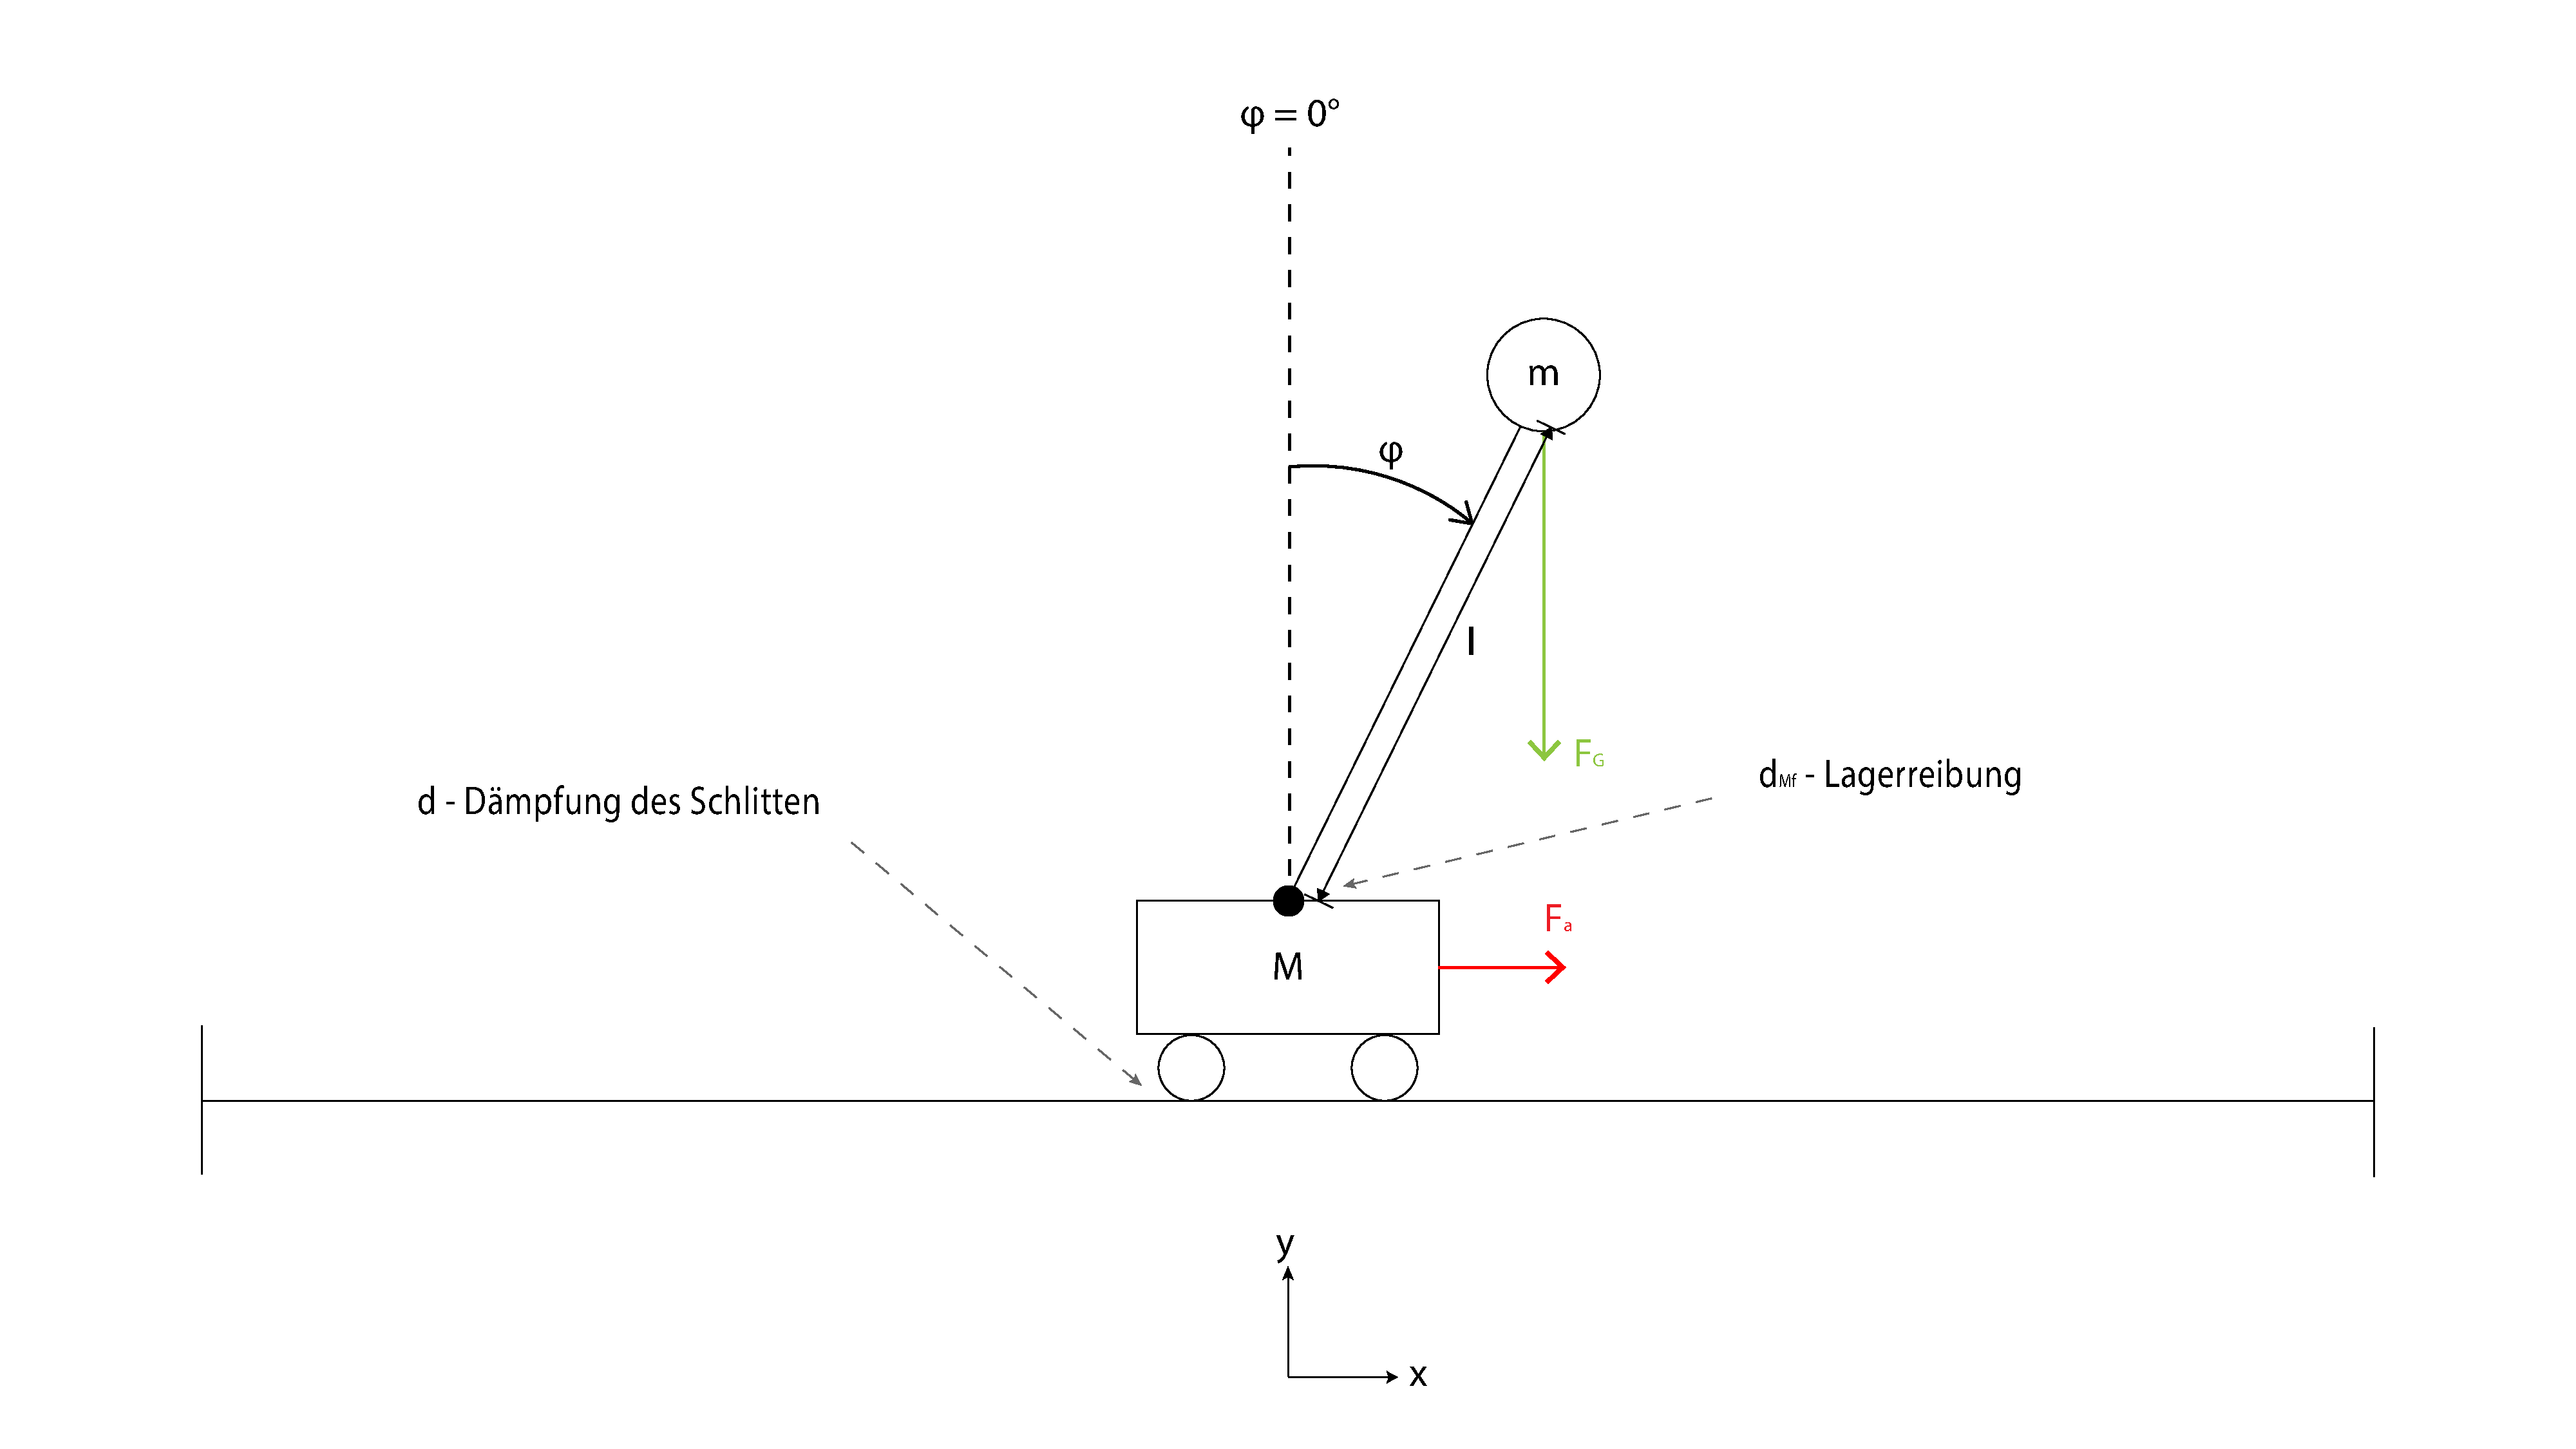
\includegraphics[width=1.0\textwidth]{Bilder/Inverses_Pendel_Skizze.pdf}}
   \caption[Skizze der Regelaufgabe]{Skizze des Aufbaus des Inversen Pendels mit Darstellung der einwirkenden Kräfte und Momente}
   \label{fig:Bild1}
\end{figure}